%!TEX root = ../report.tex

\section{IP Security (IPSec)}
IPSec provides data origin authentication and confidentiality below the connection level.
It aims to ensure that, if applied, it should neither be possible to send an IP datagram with a spoofed IP source or destination address, change the contents of the datagram nor to replay one without the receiver noticing it.
Furthermore it should not be possible to eavesdrop on the content of the packets and only little traffic flow information should leak.
Sender, receiver and intermediate nodes should be able to determine the required protection of an IP packet according to a local security policy.
If this policy is not met, packets should be dropped.

\subsection{Architecture}
\begin{figure}[h]
  \centering
  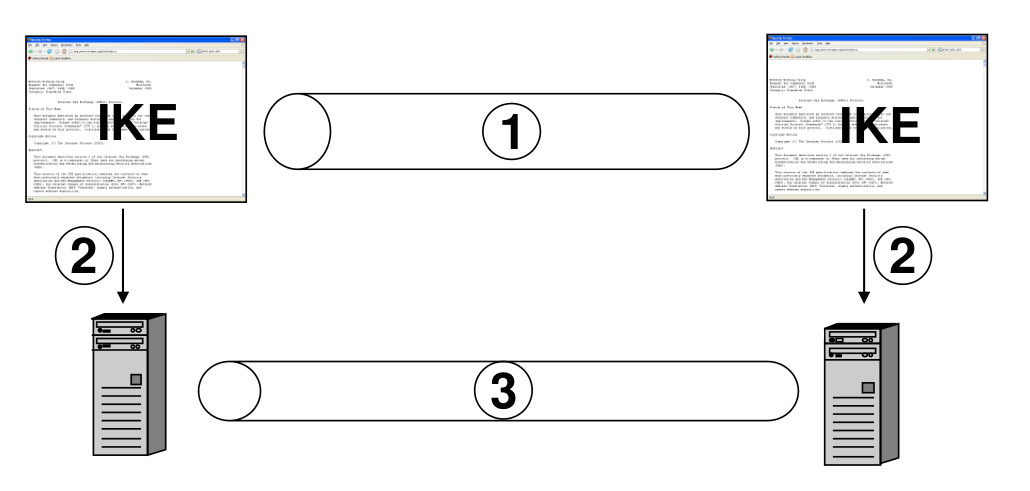
\includegraphics[width=.8\textwidth]{figures/ipsec_arch.png}
  \caption{IPSec Architecture}\label{fig:ipsec_arch}
\end{figure}
IPsec basically works in three steps (shown in Figure~\ref{fig:ipsec_arch}).
The first step is to establish a key that will be used by the cryptographic functions later on.
These keys then have to be hand over to the IPSec algorithms which can ensure data integrity with the help of an \textbf{Authentication Header (AH)} or encryption and authentication with the \textbf{Encapsulating Security Payload (ESP)} protocol.
So a secure communication is set up.\\

This communication can happen in one of two modes, tunnel and transport mode.
\textbf{Transport mode} can only be used for communications between two communication end-points which have to be equal to the cryptographic endpoints.
We define communication endpoints here as the actual communication partners and cryptographic endpoints as the points where IPSec is applied.
In \textbf{tunnel mode}, at least one cryptographic endpoint is not a communication endpoint.
The cryptographic endpoints in this mode are called security gateways.
Tunneled packets will have two IP Headers, one for the communication between the security gateways and one for the actual endpoints.
These two header differ in the source and destination IP addresses.\\

IPSec uses two databases to store relevant informations.
The \textbf{Security policy database (SPD)} stores information of how and to which IP packets security services should be applied.
As identification of relevant packets \textbf{traffic selectors (TS)} are used.
These consist of the IP source address, IP destination address, a name (DNS name, X.500 name, \dots) and a protocol identifier.
Note here that including the protocol allows applying IPsec differently for different applications.
The information of how to use security services to the now identified packets is called \textbf{security policy (SP)}.
These contain information about the security protocol (AH or ESP), protocol mode (tunnel or transport), the action to take (discard, secure, bypass) and other parameters like the policy lifetime.
SPs have to be set up by the system administrator.
The second database used is called \textbf{security associations database (SAD)} and contains informations about how to process incoming and outgoing packets, i.e.\ how to apply encryption/authentication algorithms.
Every entry, called \textbf{security association (SA)}, is identified by an \textbf{security parameter index (SPI)}.
This index is specified by the receiving end during the SA negotiations (in step one of the previously described model) and will be sent included in the IPSec protocol headers.
The security associations store informations about the IP source and destination address, the security protocol (AH or ESP), the current sequence number, the algorithms and keys used for the security protocols (and other data needed like an IV), the SA lifetime, the protocol mode (tunnel or transport) and other relevant informations.
SAs are set either manually or with the help of the key establishment protocols where latter is more advisable usually.
Note that one SA has to be set up for every direction of the communication.\\

To guarantee replay protection, IPSec uses sequence numbers.
This sequence number is initially set to 0 when the SA is set up and increased with every packet.
The receiver of a packet checks on receipt if the sequence number lays in a field of feasible sequence numbers.
If the number of the packet is bigger than the highest number in the window, the window is advanced and the packet is accepted.
If it is in the range of the window, it is simply accepted and the window keeps as is.
If it is smaller, the packet will be discarded.
The recommended window size is 64 packets and 32 is the minimum.

\subsection{Packet Processing}
\begin{figure}[H]
  \centering
  \begin{subfigure}{.4\textwidth}
    \centering
    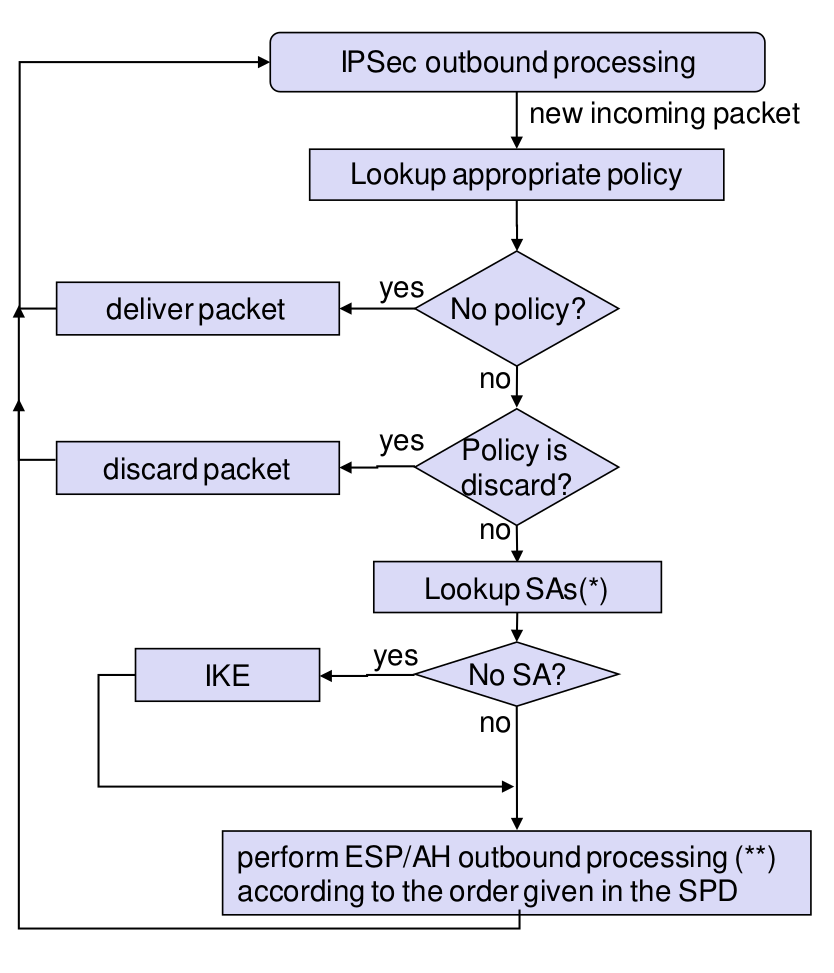
\includegraphics[width=\textwidth]{figures/ipsec_processing_outgoing.png}
    \caption{Outgoing}\label{fig:ipsec_processing_outgoing}
  \end{subfigure}
  \hspace{.1\textwidth}
  \begin{subfigure}{.4\textwidth}
    \centering
    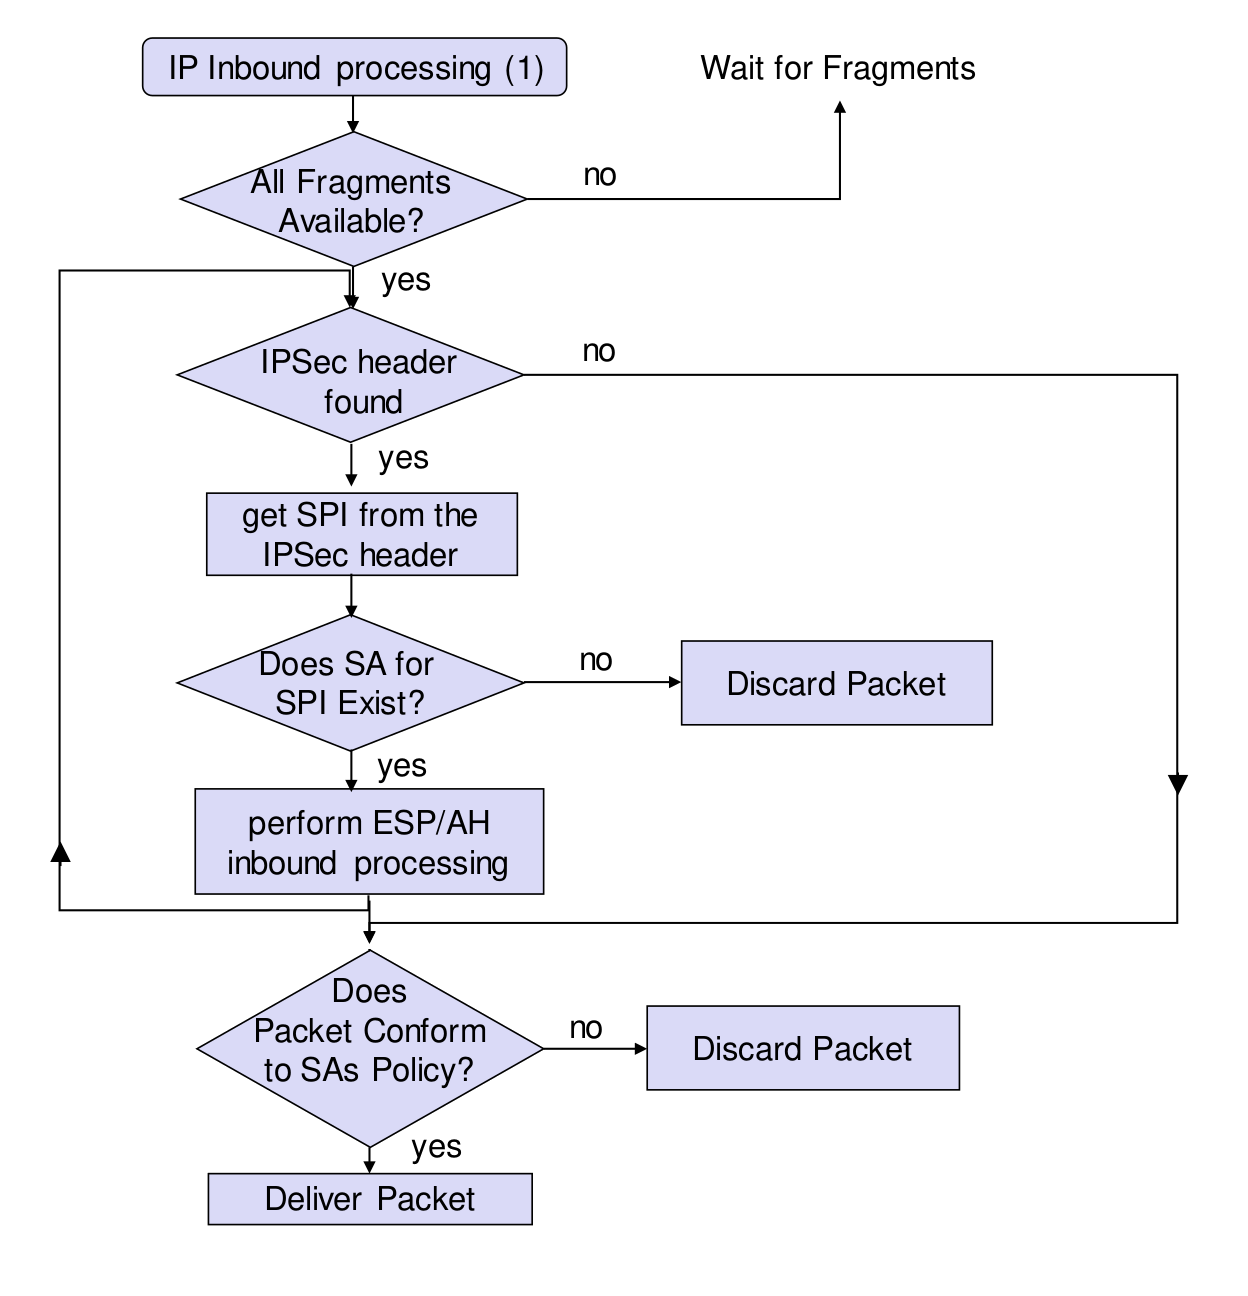
\includegraphics[width=\textwidth]{figures/ipsec_processing_incoming.png}
    \caption{Incoming}\label{fig:ipsec_processing_incoming}
  \end{subfigure}
  \caption{IPSec Packet Processing}\label{fig:ipsec_processing}
\end{figure}
Figure~\ref{fig:ipsec_processing} shows the processing process of incoming and outgoing packets.
Note that in Figure~\ref{fig:ipsec_processing_outgoing} incoming packets mean incoming from the layer above not from a communication partner.

\subsection{Encapsulating Security Protocol (ESP)}
ESP is a generic security protocol that provides replay protection and confidentiality and/or data origin authentication.
The header, shown in Figure~\ref{fig:esp_header}, follows either an IP header or an AH header whose next-header field should state $50$ for ESP\@.
\begin{figure}[h]
  \centering
  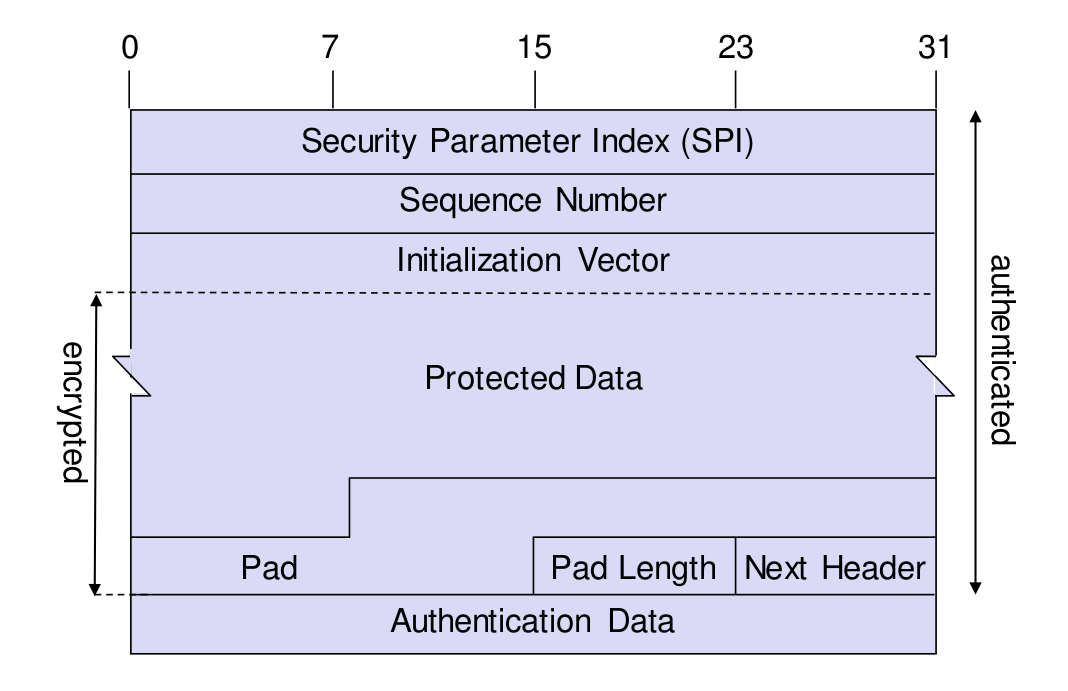
\includegraphics[width=.7\textwidth]{figures/esp_header.png}
  \caption{ESP Header}\label{fig:esp_header}
\end{figure}

ESP uses an encrypt-then-authenticate methodology.

How an entire IP packet looks like in transport and tunnel mode is shown in Figure~\ref{fig:esp_ip_packet}.
\begin{figure}[h]
  \centering
  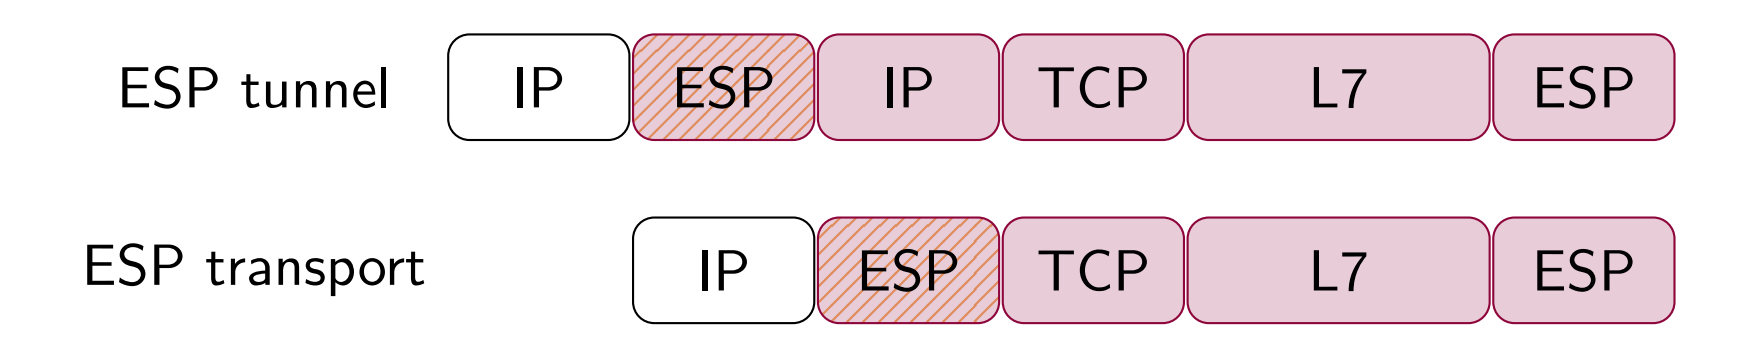
\includegraphics[width=.9\textwidth]{figures/esp_ip_packet}
  \caption{ESP IP packet}\label{fig:esp_ip_packet}
\end{figure}

\subsection{Authentication Header (AH)}
AH is a generic security protocol that provides replay protection and data origin authentication.
The AH, shown in Figure~\ref{fig:ah_header}, directly follows an IP header whose next-header field is set to $51$ for AH\@.
\begin{figure}[h]
  \centering
  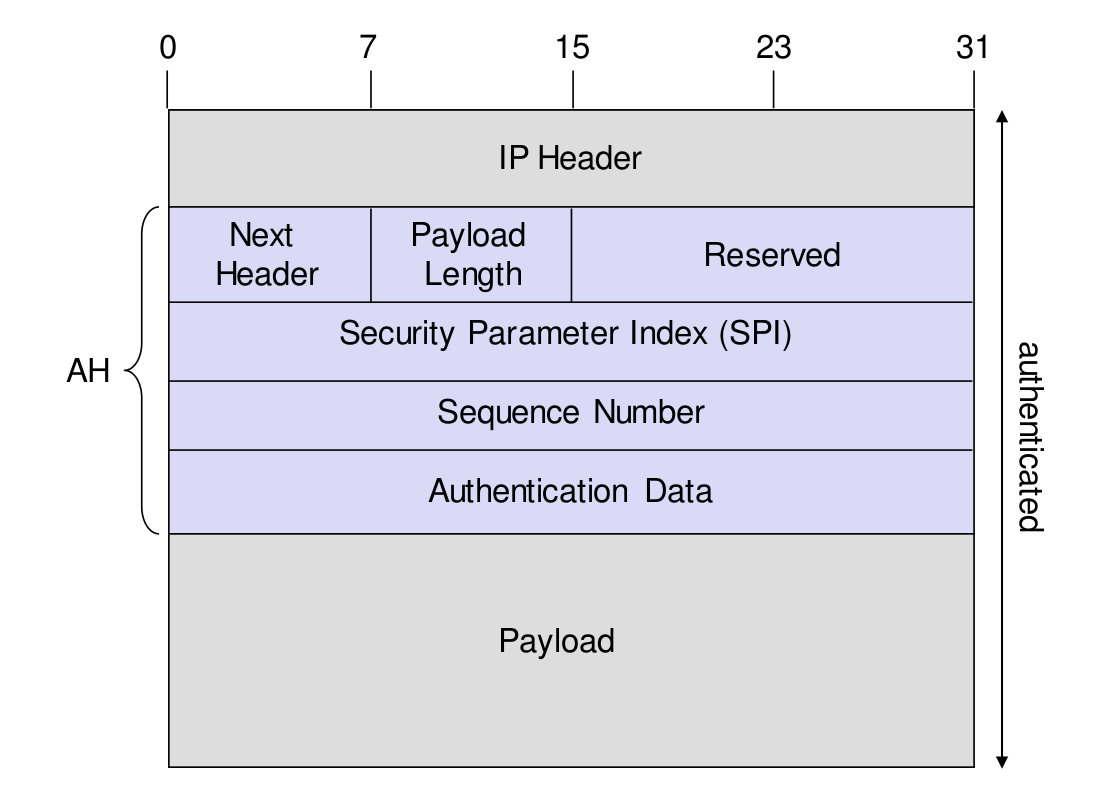
\includegraphics[width=.7\textwidth]{figures/ah_header.png}
  \caption{Authentication Header}\label{fig:ah_header}
\end{figure}
If both ESP and AH are applied by one entity, ESP is usually applied first which has the advantage that the ESP header is also protected by AH\@.
Although the AH also protects the outer IP header, some fields must not be protected, i.e.\ set to $0$ when computing authentication, because they will change during transmit.
These fields are TOS, flags, fragment offset, TTL and the header checksum.

How an entire IP packet looks like in transport and tunnel mode is shown in Figure~\ref{fig:ah_ip_packet}.
\begin{figure}[h]
  \centering
  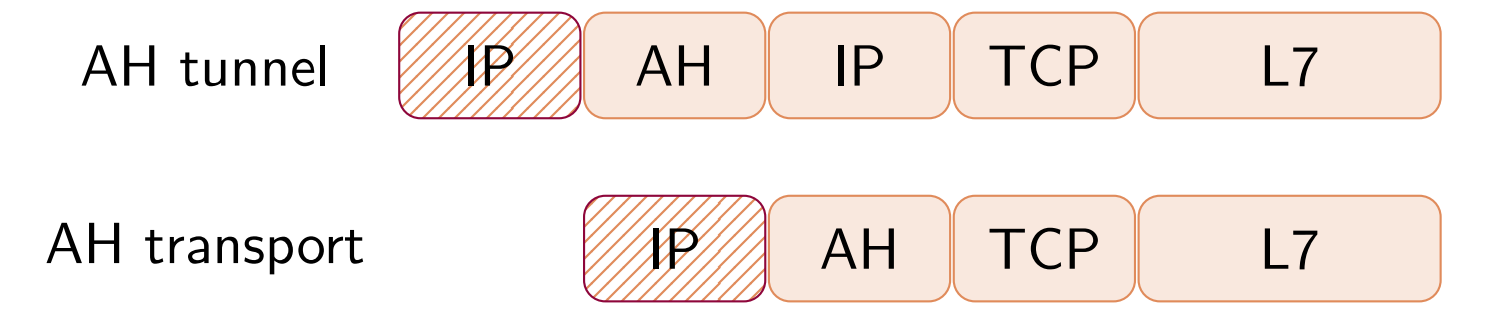
\includegraphics[width=.8\textwidth]{figures/ah_ip_packet.png}
  \caption{AH IP packet}\label{fig:ah_ip_packet}
\end{figure}

\subsection{Internet Key Exchange (IKE)}
IKE provides a unified authentication and key establishment protocol that tries to achieve a reasonable trade-off between features to choose from, overall protocol complexity and reasonable security under a realistic threat model.
It runs on UDP port 500 and 4500 with a latency of 2 round trips in the common case, so 4 messages.
In the following we will talk about IKEv2, the first version was replaced by it to its poor specification.\\

IKEv2 communications consist of message pairs, called exchange, where every request requires a response.
A protocol run always starts with two exchanges, IKE\_SA\_INIT and IKE\_AUTH\@.
IKE\_SA\_INIT negotiates the security parameters for an IKE security association (IKE\_SA) and sends nonces and Diffie-Hellman values.
An IKE\_SA is a set of security associations used to encrypt and integrity-protect all remaining IKE exchanges.
IKE\_AUTH authenticates the previously sent messages, transmits identities, proves knowledge of the secrets corresponding to the identities and creates a first CHILD\_SA\@.
CHILD\_SAs are sets of security associations used to encrypt and/or integrity-protect data with AH/ESP.\\
Additionally to these two exchanges an CREATE\_CHILD\_SA (create new child SA, rekeying) or an INFORMATIONAL exchange (keep-alive, deleting SA, errors, \dots) are possible.

\subsubsection{IKE\_SA\_INIT Exchange}
Figure~\ref{fig:ike_sa_init} shows the IKE\_SA\_INIT exchange where $SA_{I1}$ are the cryptographic suites which the initiator supports, $SA_{R1}$ the responder's chosen suite, $KE_I$ and $KE_R$ the initiators and responders public Diffie-Hellman values, $N_I$ and $N_R$ nonces and $CERTREQ$ an optional certificate request payload used for authentication via certificates.
\begin{figure}[H]
  \centering
  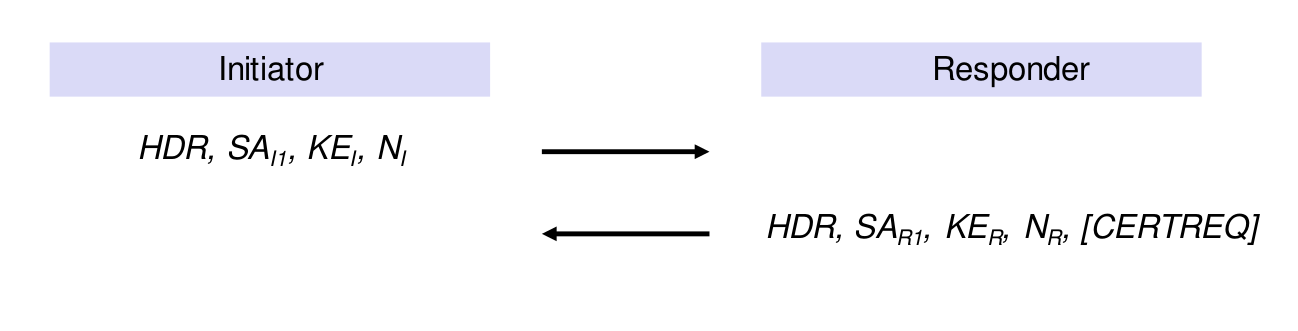
\includegraphics[width=.8\textwidth]{figures/ike_sa_init.png}
  \caption{IKE\_SA\_INIT Exchange}\label{fig:ike_sa_init}
\end{figure}

IKE\_SA\_INIT negotiates four cryptographic algorithms: encryption, integrity-protection, Diffie-Hellman and pseudo-random function ($prf(K,S)$, cryptographic hash function).
The prf is used to generate the key material for the subsequent IKE\_SA and CHILD\_SAs.
The amount of key material needed might actually be greater than the return value of prf.
For this reason prf is used subsequently according to the following rule.
\begin{equation*}
  \begin{aligned}
    prf^+(K,S) & = T1~|~T2~|~\dots\\
    T1 & = prf(K,S~|~0x01)\\
    T2 & = prf(K,T1~|~S~|~0x02)\\
    \dots
  \end{aligned}
\end{equation*}
The DH exchange in IKE\_SA\_INIT enables both parties to generate a shared key $SKEYSEED = prf(N_I~|~N_R, g^{IR})$.
This seed is then used to calculate 7 different keys 
\begin{equation*}
  SK_d~|~SK_{ai}~|~SK_{ar}~|~SK_{ei}~|~SK_{er}~|~SK_{pi}~|~SK_{pr} = prf^+(SKEYSEED, N_i~|~N_r~|~SPI_i~|~SPI_r)
\end{equation*}
where $SK_{ai}$ and $SK_{ar}$ are used for integrity protection of subsequent IKEv2 exchanges, $SK_{ei}$ and $SK_{er}$ for encrypting and decrypting messages in subsequent IKEv2 exchanges, $SK_d$ for deriving new keys for the CHILD\_SAs established with this IKE\_SA and $SK_{pi}$ and $SK_{pr}$ for generating AUTH payloads in the IKE\_AUTH exchange.\\

Note that the SKEYSEED and thus all derived keys unauthenticated at that point.
To resolve this issue, the IKE\_AUTH exchange is used.

\subsubsection{IKE\_AUTH Exchange}
Figure~\ref{fig:ike_auth} shows the IKE\_AUTH exchange where $\{\dots \}_{SK}$ indicates that these payloads are encrypted and authenticated and $ID_I$ and $ID_R$ are the identities of the communication partners.
\begin{figure}[h]
  \centering
  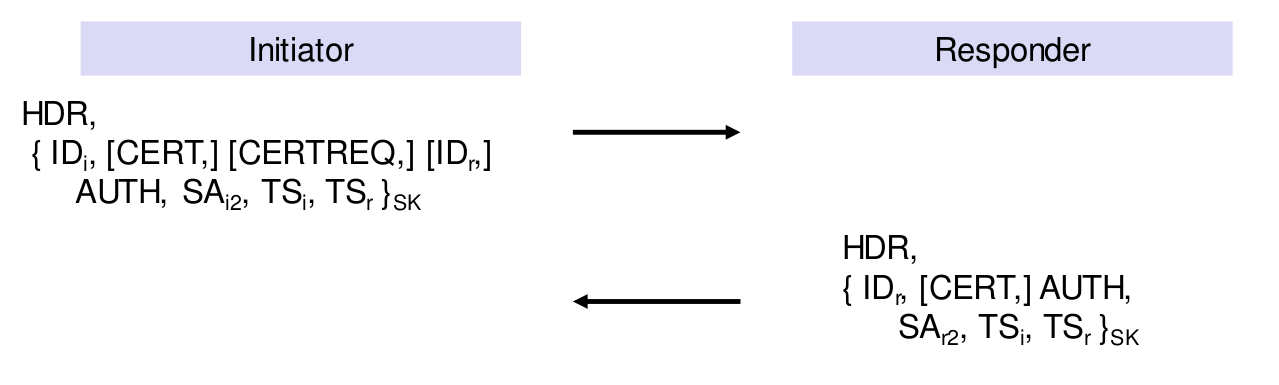
\includegraphics[width=.8\textwidth]{figures/ike_auth.png}
  \caption{IKE\_AUTH Exchange}\label{fig:ike_auth}
\end{figure}
The AUTH payload is used to prove the knowledge of the secret corresponding to the ID of the corresponding party and to authenticate the corresponding message in the IKE\_SA\_INIT exchange.
The initiator therefore authenticates the whole payload of their IKE\_SA\_INIT message, the responders nonce and $prf(SK_{pi}, ID_i')$.
The responder does the same for his IKE\_SA\_INIT message, the initiator's nonce and $prf(SK_{pr},ID_r')$.\\

Figure~\ref{fig:ike_keys} shows the usage of the generated keys again.
\begin{figure}[h]
  \centering
  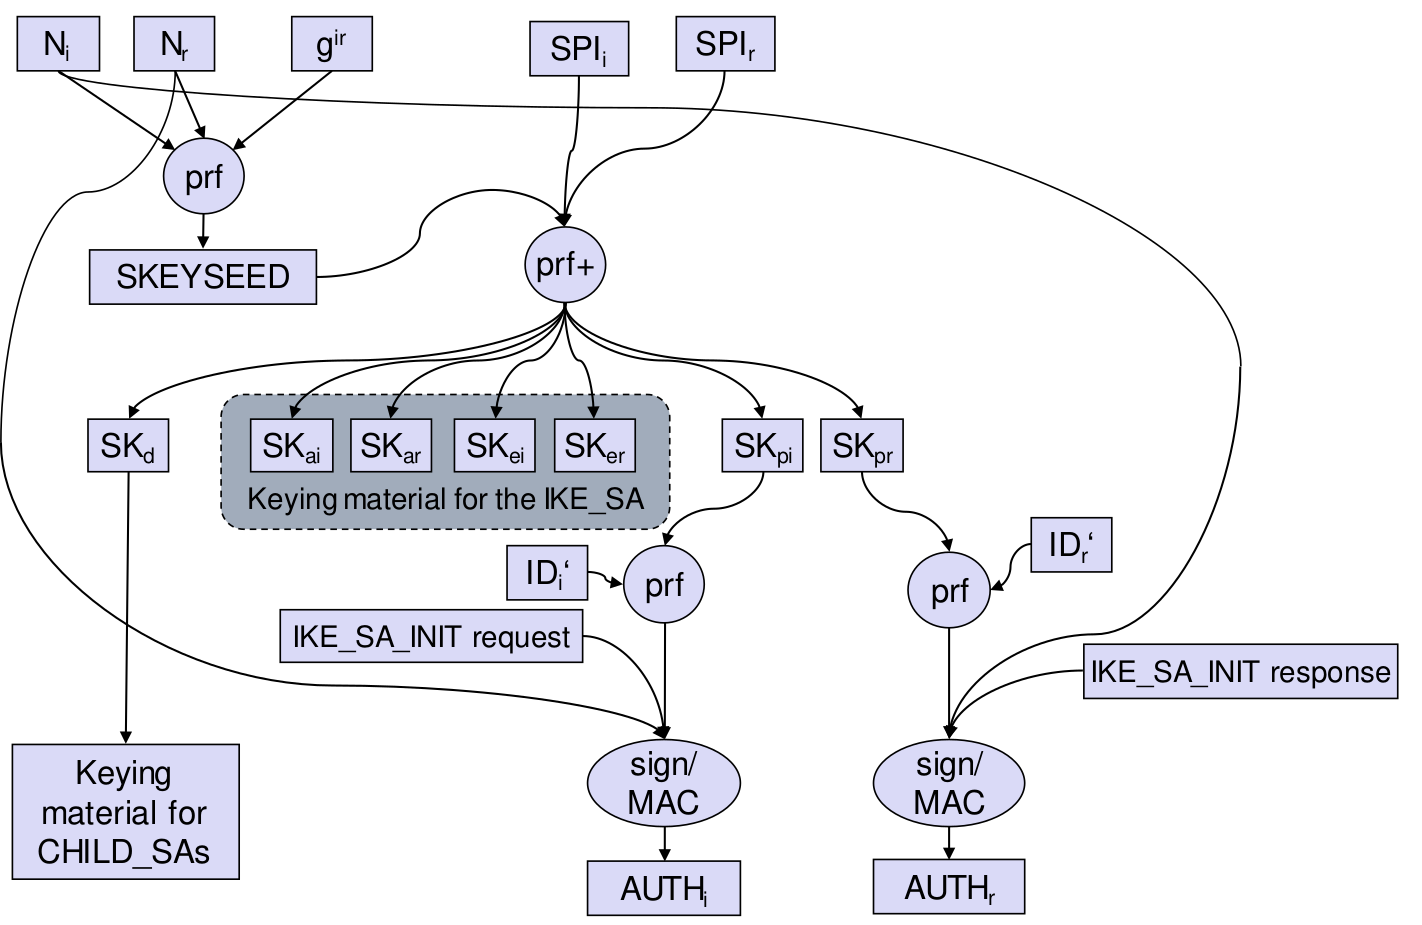
\includegraphics[width=.8\textwidth]{figures/ike_keys.png}
  \caption{IKEv2 Key Usage}\label{fig:ike_keys}
\end{figure}

\subsubsection{CREATE\_CHILD\_SA Exchange}
Figure~\ref{fig:ike_create_child_sa} shows the CREATE\_CHILD\_SA exchange where $N$ is a notify payload used for re-keying, $SA$ are SA offer(s), $N_I$ and $N_R$ nonces, $KE_I$ and $KE_R$ optional DH values and $TS_I$ and $TS_R$ proposed traffic selector payloads.
\begin{figure}[h]
  \centering
  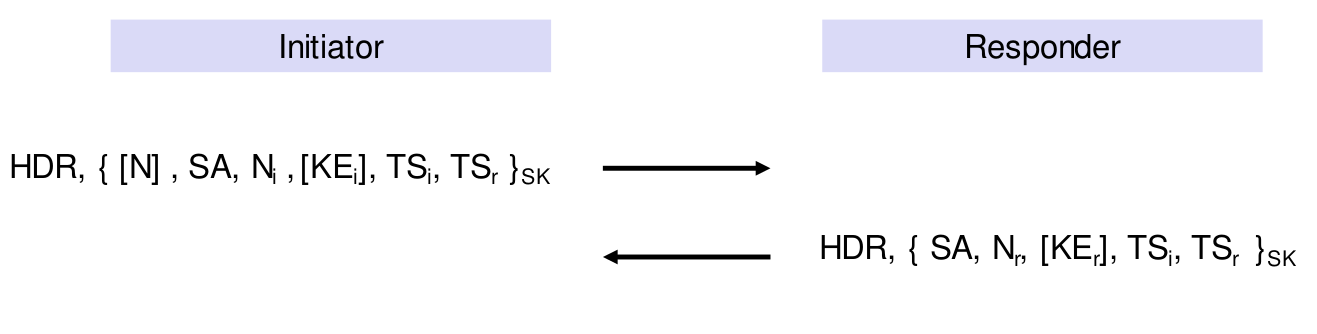
\includegraphics[width=.8\textwidth]{figures/ike_create_child_sa.png}
  \caption{IKE\_CREATE\_CHILD Exchange}\label{fig:ike_create_child_sa}
\end{figure}

Note that a single (CREATE\_)CHILD\_SA negotiation may result in multiple SAs.

\subsubsection{Protection against Flooding Attacks}
Flooding Attack prevention in IKEv2 is handled in that the responder may switch to an alternative protocol, that involves three exchanges in case large numbers of half open IKE\_SAs are present.
This protocol involves sending a cookie similar to TCP SYN cookies.

\subsubsection{Message Format}
Figure~\ref{fig:ike_message_format} shows the structure of IKE messages.
Some things to note here:
\begin{itemize}
  \item An SA payload may contain multiple proposals where each contains a set of security protocols with the corresponding algorithms.
  \item Proposals are ordered according to preference.
  \item The first proposal must have the proposal number 1, all following a higher or equal one
  \item If two proposals structures have the same number, it means that the proposal consists of the first and the second structure
\end{itemize}
\begin{figure}[h]
  \centering
  \begin{subfigure}{.4\textwidth}
    \centering
    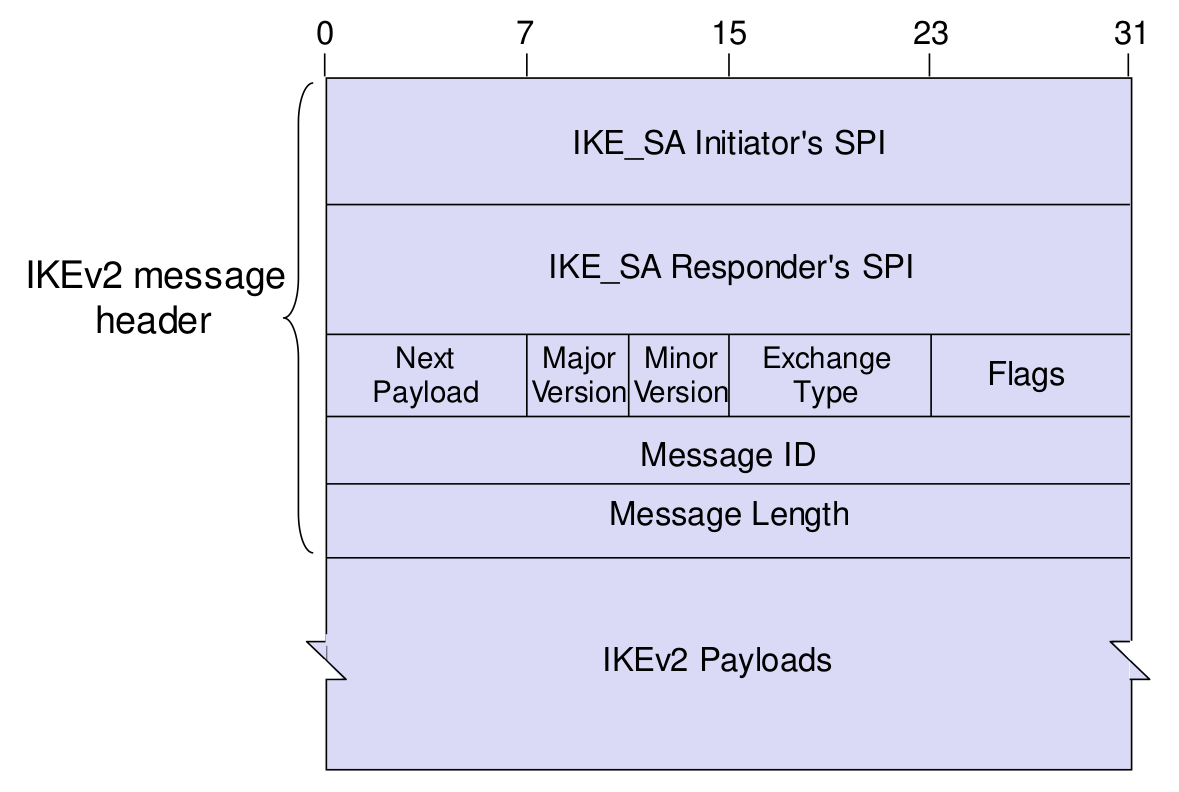
\includegraphics[width=\textwidth]{figures/ike_message_format.png}
    \caption{General}\label{fig:ike_general_message}
  \end{subfigure}
  \hspace{.05\textwidth}
  \begin{subfigure}{.4\textwidth}
    \centering
    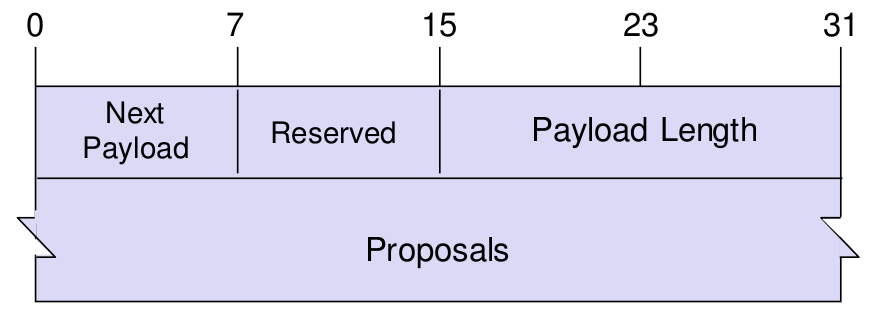
\includegraphics[width=\textwidth]{figures/ike_negotiation_structure.png}
    \caption{Negotiation}\label{fig:ike_negotiation_format}
  \end{subfigure}
  \begin{subfigure}{.4\textwidth}
    \centering
    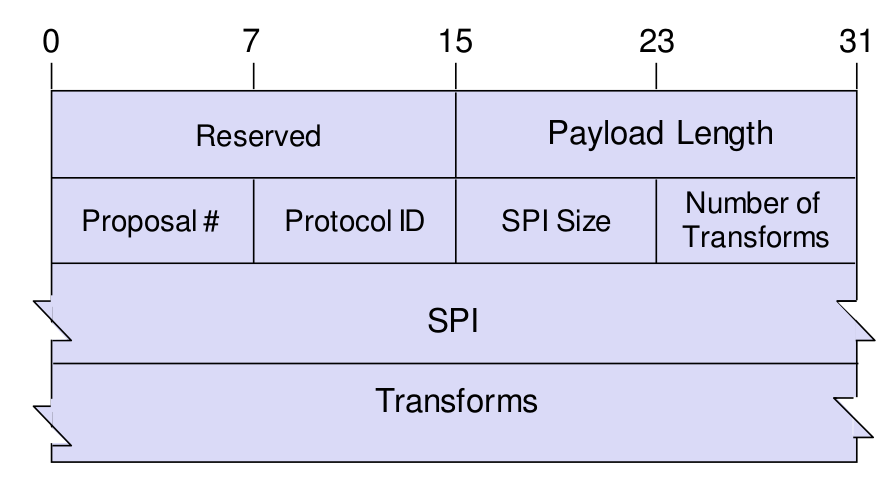
\includegraphics[width=\textwidth]{figures/ike_proposal_structure.png}
    \caption{Proposal}\label{fig:proposal_structure}
  \end{subfigure}
  \hspace{.05\textwidth}
  \begin{subfigure}{.4\textwidth}
    \centering
    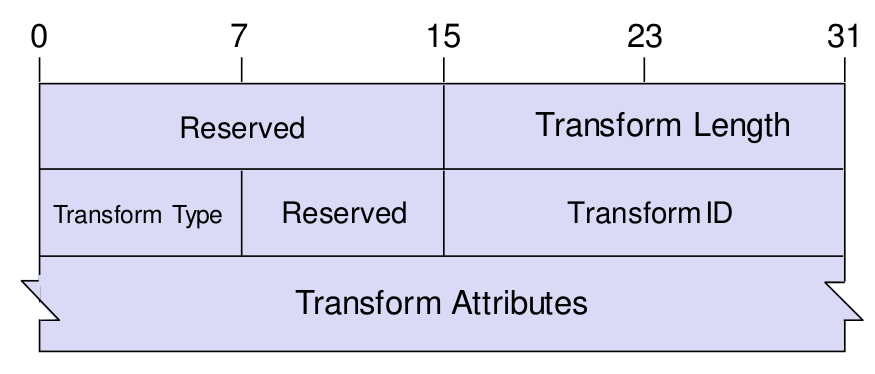
\includegraphics[width=\textwidth]{figures/ike_transform_structure.png}
    \caption{Tranforms}\label{fig:ike_transform_structure}
  \end{subfigure}
  \caption{IKE Message Format}\label{fig:ike_message_format}
\end{figure}
